%%%%%%%%%%%%%%%%%%%%%%%%%%%%%%%%%%%%%%%%%%%%%%%%%%%%%%%%%%%%%%%%%%%%%%%%%%%%%%%
% Neuroimage-like layout
\documentclass[5p]{elsarticle}
\usepackage{amsmath,amsfonts,amssymb}
\usepackage{bm}
\usepackage{algorithm}
\usepackage{algorithmic}
\usepackage{url}
\usepackage[breaklinks=true,letterpaper=true,colorlinks,bookmarks=false]{hyperref}
\usepackage[table]{xcolor}

\definecolor{deep_blue}{rgb}{0,.2,.5}
\definecolor{dark_blue}{rgb}{0,.15,.5}

\hypersetup{pdftex,  % needed for pdflatex
  breaklinks=true,  % so long urls are correctly broken across lines
  colorlinks=true,
  linkcolor=dark_blue,
  citecolor=deep_blue,
}

% Float parameters, for more full pages.
\renewcommand{\topfraction}{0.9}        % max fraction of floats at top
\renewcommand{\bottomfraction}{0.8}     % max fraction of floats at bottom
\renewcommand{\textfraction}{0.07}      % allow minimal text w. figs
%   Parameters for FLOAT pages (not text pages):
\renewcommand{\floatpagefraction}{0.6}  % require fuller float pages
%    % N.B.: floatpagefraction MUST be less than topfraction !!


\def\B#1{\mathbf{#1}}
%\def\B#1{\bm{#1}}
\def\trans{^\mathsf{T}}
% A compact fraction
\def\slantfrac#1#2{\kern.1em^{#1}\kern-.1em/\kern-.1em_{#2}}

%%%%%%%%%%%%%%%%%%%%%%%%%%%%%%%%%%%%%%%%%%%%%%%%%%%%%%%%%%%%%%%%%%%%%%%%%%%%%%%%
\begin{document}

%\title{Comparing Connectomes Between Populations}
\title{Learning and comparing functional connectomes between populations}


\author[parietal,unicog,cea]{Ga\"el Varoquaux\corref{corresponding}}
\author[cmi,nki]{R. Cameron Craddock}

\cortext[corresponding]{Corresponding author}

\address[parietal]{Parietal project-team, INRIA Saclay-\^ile de France}
\address[unicog]{INSERM, U992}
\address[cea]{CEA/Neurospin b\^at 145, 91191 Gif-Sur-Yvette}
\address[cmi]{Child Mind Institute, New York, New York}
\address[nki]{Nathan Kline Institute for Psychiatric Research, Orangeburg, New York}

\begin{abstract}
    We are the champion... of the world

    Scope: rest and task-based studies. But focusing on fMRI.
\end{abstract}

\begin{keyword}
    Functional connectivity, connectome, group study, effective
    connectivity, fMRI, resting-state
\end{keyword}

\maketitle
%%%%%%%%%%%%%%%%%%%%%%%%%%%%%%%%%%%%%%%%%%%%%%%%%%%%%%%%%%%%%%%%%%%%%%%%%%%%%%%%

\sloppy % Fed up with messed-up line breaks
\section{Introduction}

Review paper giving technical guidelines.

BOLD signal during rest is typically just 5-10\% lower than during task-based
experiments (cite Raichle,  Mintun, Annu. Rev. Neurosci. 29, 449–476 (2006).)

Define what we call a functional connectome, and the term \emph{graph},
as well as its relation with an adjacency matrix.

Define a functional network

Define on-going vs evoked activity


%%%%%%%%%%%%%%%%%%%%%%%%%%%%%%%%%%%%%%%%%%%%%%%%%%%%%%%%%%%%%%%%%%%%%%%%%%%%%%%

\section{Estimating functional connectomes}

Here we discuss strategies to infer connectomes from functional brain
imaging data. We start with the choice of nodes \emph{i.e.} regions,
followed by signal extraction, and the estimation of graphs.

%------------------------------------------------------------------------------
\subsection{Defining regions}

The choice of regions of interests (ROIs) that defines the nodes of the
graphs can be very important both in the estimation of connectomes and
for group comparison \cite{wang2009}. Unsurprisingly, simulations have
shown that extracting signal from ROIs that did not match functional
units would lead to incorrect graph extraction \cite{smith2011}.
%
Different strategies coexist. While dense parcellations approaches cover
a large fraction of the brain \cite{achard2006, varoquaux2010c,
wang2009}, this coverage can be traded off to focus on some specific
regions, in favor of increased functional specificity and thus better
differentiation across networks \cite{greicius2003, fair2009,
varoquaux2010b, lewis2009, fransson2008, shirer2012}. In addition, while
ROIs and most often defined as a hard selection of voxels, it is also
possible to use a \emph{soft} definition, attributing weights as with
probabilistic atlases, or spatial maps of functional networks extracted
from techniques such as independent component analysis (ICA).

% XXX: discuss tradeoffs in the number of regions

\paragraph{Regions from atlases}
%
Atlases can be used to define full-brain parcellations. The most popular
choice is probably the AAL atlas \cite{tzourio-mazoyer2002a}, that
benefits from an SPM toolbox. However, it suffers from major
shortcomings; namely that \emph{i)} it was defined on a single subject
and thus does does not reflect inter-subject variability and \emph{ii)}
focuses on labeling large anatomical structures and does not match
functional layout --for instance only two regions describe the medial
part of the frontal lobe. Multi-subject probabilistic altases such as the
Harvard-Oxford atlas distributed with FSL \cite{smith2004} or the
sulci-based structural atlas used in \cite{varoquaux2010c} mitigate the
first problem, and the high number of regions defined using sulci also
somewhat circumvent the second problem (see
fig.\,\ref{fig:parcellations}).


\paragraph{Defining regions from the literature}
%
Regions can be defined from previous studies, informally or with
systematic meta-analysis. This strategy is used to define the main
resting-state networks, such as the default mode network, but may also be
useful to study connectivity in task-specific networks
\cite{grillon2012}. The common practice is to place balls of a given
radius, 5 or 10\,mm, centered at the coordinates of interest. Given that
functional networks are tightly interleaved in some parts of the cortex,
such as the parietal lobe, care must be taken not to define too many
regions that would overlap and lead to mixing of the signal.

\paragraph{FMRI-based function definition}
%
Defining regions directly from the fMRI signal brings many benefits.
First, it can capture subject-specific functional information. Second, it
also adapts to the signal at hand and it's limitations, such as
EPI-specific warps or vascular and movement artifacts that are isolated
in ICA-like approaches. The simplest approach to define task-specific
regions is to use activation maps derived from standard GLM-based
analysis in a task-driven study (see for instance \cite{poldrack2011}).
Regions are extracted by thresholding the maps, or using balls around the
activation peaks. For resting-state studies, unsupervised multivariate
analysis techniques are necessary. Clustering approaches extract
full-brain parcellations \cite{craddock2011, bellec2010, yeo2011,
thirion2006}, and have been shown to extract well-known functional
structures from rest data \cite{yeo2011}. Alternatively, decompositions
methods, such as ICA \cite{beckmann2004}, can unmixing linear
combinations of multiple effects and separate out multiple spatial maps
capturing functional networks or confounding effects. At high model
order, ICA maps define a functional parcellation \cite{kiviniemi2009}.
Extracting regions from these maps requires additional effort as they can
display fragmented spatial features and structured background noise, but
incorporating sparsity and spatial constraints in the decomposition
techniques leads to contrasted maps that outline many different
structures \cite{varoquaux2012} (see fig.\,\ref{fig:parcellations}).

%{{{------ Parcellation figure -----------------------------------------------
\begin{figure}
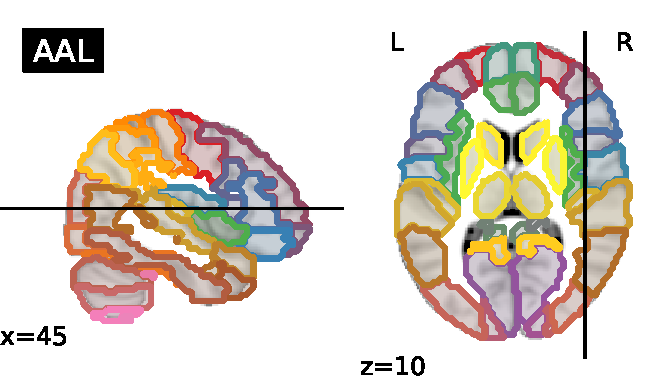
\includegraphics[width=.5\linewidth]{aal_atlas.pdf}%
\hfill%
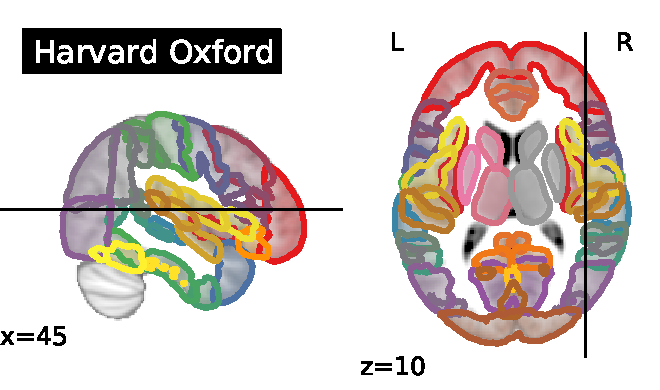
\includegraphics[width=.5\linewidth]{ho_atlas.pdf}%

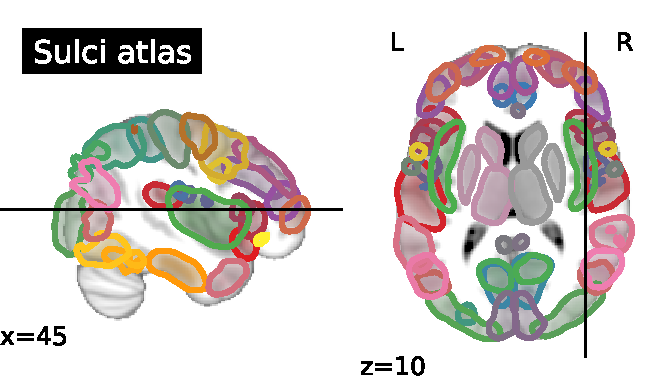
\includegraphics[width=.5\linewidth]{sulci_atlas.pdf}%
\hfill%
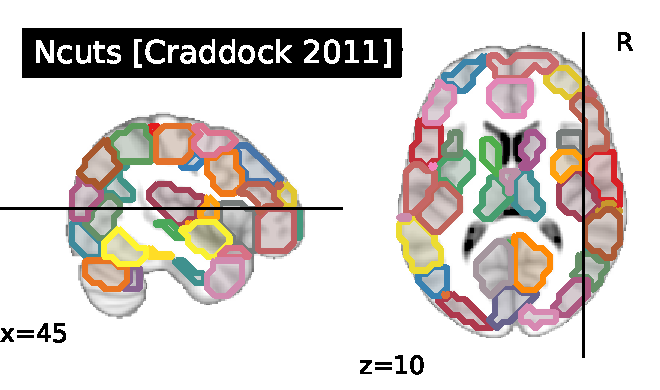
\includegraphics[width=.5\linewidth]{ncuts_atlas.pdf}%

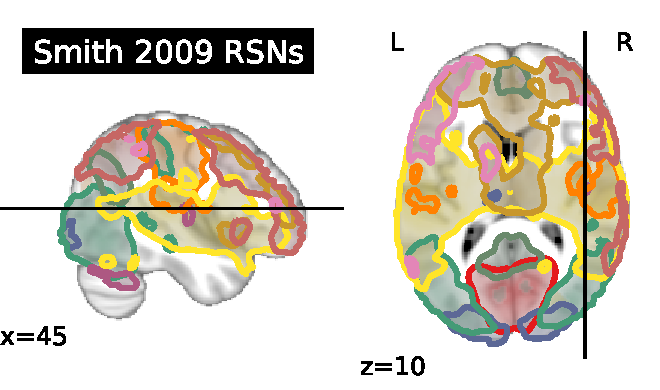
\includegraphics[width=.5\linewidth]{smith_atlas.pdf}%
\hfill%
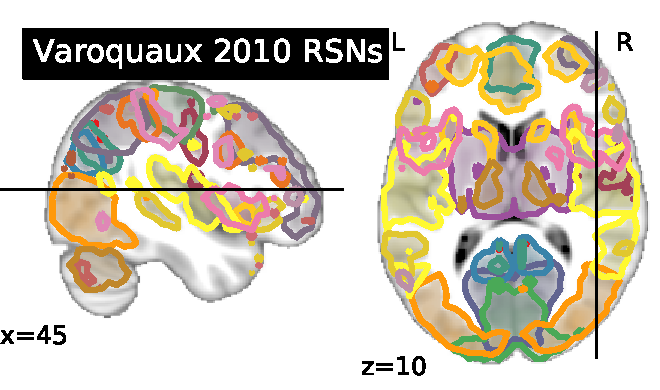
\includegraphics[width=.5\linewidth]{msdl_atlas.pdf}%

\caption{
Different full-brain parcellations: the AAL atlas
\cite{tzourio-mazoyer2002a}, the Harvard-Oxford atlas, the sucli atlas used in
\cite{varoquaux2010c}, regions extracted by Ncuts
\cite{craddock2011}, the resting-state networks extracted in
\cite{smith2009} by ICA, and in \cite{varoquaux2011} by sparse dictionary
learning.
\label{fig:parcellations}
}
\end{figure}
%---------------------------------------------------------------------------}}}

%------------------------------------------------------------------------------
\subsection{Estimating connections}

The concept of functional connectivity has be called elusive
\cite{horwitz2003}: it has many mathematical instantiations although in
essence they all strive to extract simple statistics from functional
imaging to characterize synchrony and communication between large
ensembles of neurons. Here we choose to focus on second order statistics
that can be related to Gaussian models, the simplest of which being the
correlation matrix of the signals of the different ROIs.


%{{{------ Correlation matrices figure ---------------------------------------
\begin{figure}
\newcommand{\photoframe}[1]{\setlength\fboxsep{0pt}%
{\color{black!70}\fbox{#1}\color{black}}}%
\begin{minipage}{.66\linewidth}%
    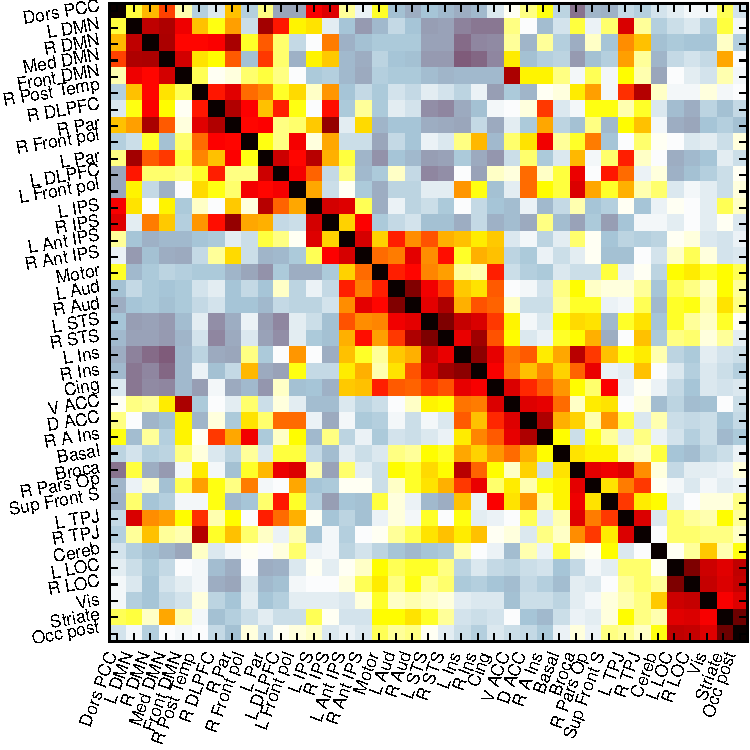
\includegraphics[width=\linewidth]{group_emp_cov.pdf}%
    \raisebox{.606\linewidth}{%
	\hspace*{-.462\linewidth}%
	\photoframe{%
	%\setlength\fboxsep{1pt}%
	\colorbox{white}{%
	\raisebox{.003\linewidth}{%
	    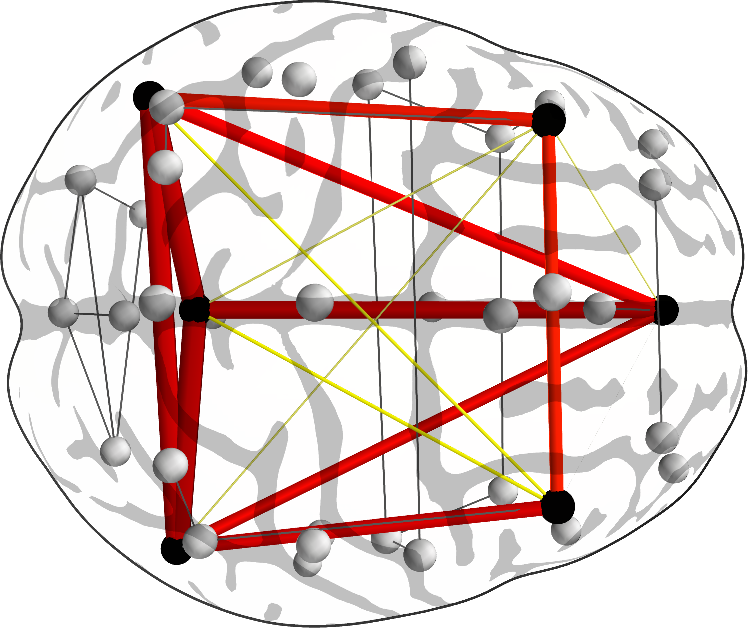
\includegraphics[width=.455\linewidth]{group_emp_cov_3d_crop}}%
	\rule{0pt}{.387\linewidth}%
	}}%
    }
\end{minipage}%
\hspace*{1pt}%
\begin{minipage}{.32\linewidth}%
    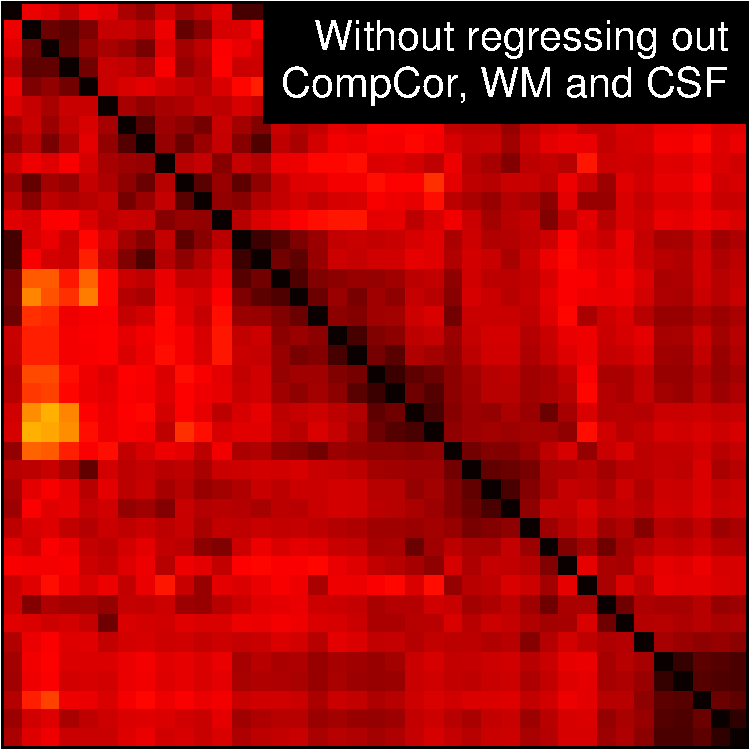
\includegraphics[width=\linewidth]{group_emp_cov_no_confounds.pdf}%

    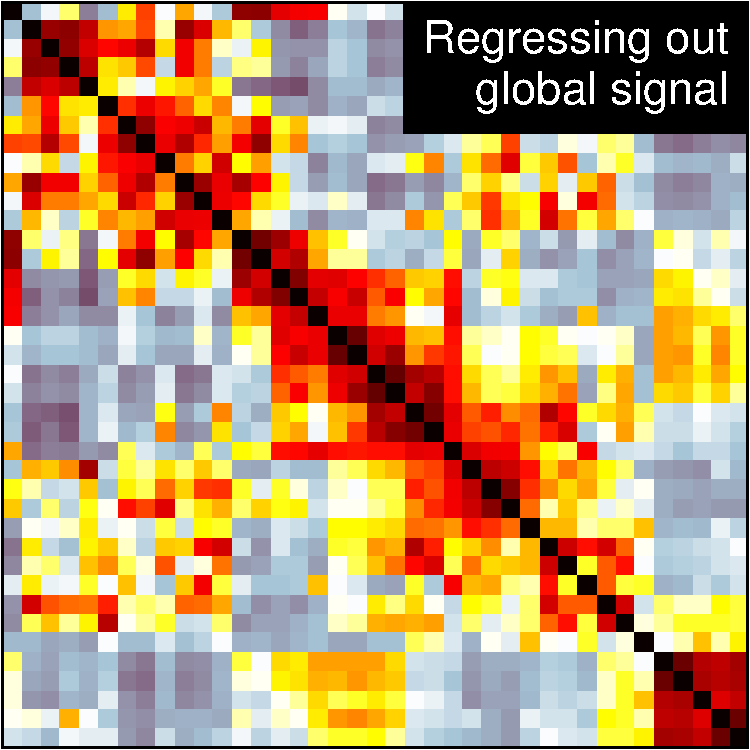
\includegraphics[width=\linewidth]{group_emp_cov_global_mean.pdf}%
\end{minipage}%

% XXX: need to give details on the dataset used here

\caption{
Correlation matrices of rest time-series extracted from the 39 main
regions of the Varoquaux 2011 \cite{varoquaux2011} parcellation -- 
Upper left: regressing out CompCor signals, as well as white matter and
CSF average signals and movement parameters. The insert shows the
connections restricted to the default mode network.
% XXX: should I outline the default mode network on the main matrix?
-- Upper right: regressing out only movement parameters. -- Lower right:
regressing out movement parameters and global signal mean.
% XXX: should this remark go here?
No frequency filtering was applied here.
\label{fig:correlation_matrices}
}
\end{figure}
%---------------------------------------------------------------------------}}}

% The following paragraph is convoluted: we start to say that rest is
% from time-series, and task from beta, we go on discussing about beta
% maps, and then we move back to rest. It might need restructuring

% Horrible sentence below

\paragraph{Signal extraction}
%
Given ROIs, the next step is to extract from them a summary measure. To
study \emph{on-going} activity, \emph{e.g.} with rest data, signal
extraction is performed from the EPI time series; however, to study
\emph{evoked} activity with task-driven studies it can be beneficial to
run a first-level analysis, enforcing specificity of the measure
extracted to the task. With slow event-related design, task-specific
functional connectivity can be captured in trial-to-trial fluctuations in
the BOLD response, estimated using a GLM analysis with one regressor per
trial \cite{grillon2012,rissman2004}. This approach, known as beta-series
regression, has been adapted for rapid event-related designs, using
multiple GLMs to optimize deconvolution of each trial \cite{mumford2012}.
With rest datasets, it is important to regress out time series capturing
movement and other sources of structured noise, to separate on-going
activity from confounding signals. In addition to removing movement
parameters estimated during preprocessing, removing linear trends, signal
extracted from the white matter and the CSF \cite{chang2009}, as well as
using the CompCor \cite{behzadi2007} procedure gives more contrasted
correlation matrices that outline functional structures better
(fig.\,\ref{fig:correlation_matrices}). Filtering high frequencies is
often recommended, based on the initial observation that neural-related
signal are observed below 0.1\,Hz \cite{cordes2001,biswal1995}. While
high-pass and low-pass filtering decrease the impact of some confounds,
recent studies have shown that information on neural processes is present
in the full spectrum of frequencies observed
\cite{smith2012,vanoort2012}. Regressing out a good choice of confound
signals is more specific than frequency filter, and in our experience
gives more contrasted correlation matrices\footnote{Note that naive use
of filtering can induce spurious correlations \cite{davey2012}.}.

Finally, it is important to keep in mind that using resting-state to
study on-going activity is fragile to confounds such as movement
\cite{vandijk2012,power2011} or scanner noise, and probably more so than
activation studies as it is harder to control the specificity of the
signal extracted. Special care must be taken in preprocessing strategies
\cite{vandijk2010,satterthwaite2012}.
%
In addition, improved specificity to BOLD signal can be enforced by
using only signal in voxels near gray-matter tissues. For this purpose,
we suggest summarizing the signal in an ROI by a mean of the different voxels
weighted by the subject-specific gray matter probabilistic segmentation,
as output by \emph{e.g.} SPM's segmentation tool \cite{ashburner2005}.

% Regressing out task?? Skipping for lack of space

\paragraph{Correlation and partial correlations}
%
Functional connectivity between the ROIs can be measured by computing the
correlation matrix of the extracted signals. An important and often
neglected point is that the sample correlation matrix, \emph{i.e.} the
correlation matrix obtained by plugging the observed signal in the
correlation matrix formula, is not the population correlation matrix,
\emph{i.e.} the correlation matrix of the data-generating process. If the
number of measurements was infinite, the two would coincide, however if
this number is not large compared to the number of connection (that
scales as the square of the number of ROIs), the sample correlation
matrix is a poor estimate of the underlying population correlation matrix.
In other words, the sample correlation matrix captures a lot of sampling
noise, intrinsic randomness that arises in the estimation of correlations
from short time series. Conclusions drawn from the sample correlation
matrix can easily reflect this estimation error.

Varoquaux \emph{et al.} \cite{varoquaux2010c} and Smith \emph{et al.}
\cite{smith2011} have shown respectively on rest fMRI and on realistic
simulations that a good choice of correlation matrix estimator could
recover the connectivity structure, where the sample correlation matrix
would fail. In general, the choice of a better estimate depends on the
settings and the end goals \cite{varoquaux2012,varoquaux2010b}, however
the Ledoit-Wolf shrinkage estimate \cite{ledoit2004} is a simple,
computationally-efficient, and parameter-less alternative that performs
uniformly better than the sample correlation matrix
\cite{varoquaux2012,varoquaux2010c} and should always be prefered.

Remark: difference between covariance and correlation matrix.

partial correlation, sparse iCov. \cite{smith2011,varoquaux2010b}. 

Give intuition on partial correlation/inverse covariance.

Remark that partial correlations consistently have no negative values.

Variety
of estimation strategies for sparse iCov, that have an impact on the
resulting network \cite{varoquaux2012}\footnote{Better estimation
algorithm is recent Honorio paper.}. Discuss setting the regularization
parameter.


%{{{------ Precision matrices figure -----------------------------------------
\begin{figure}
\newcommand{\photoframe}[1]{\setlength\fboxsep{0pt}%
{\color{black!70}\fbox{#1}\color{black}}}%
\begin{minipage}{.66\linewidth}%
    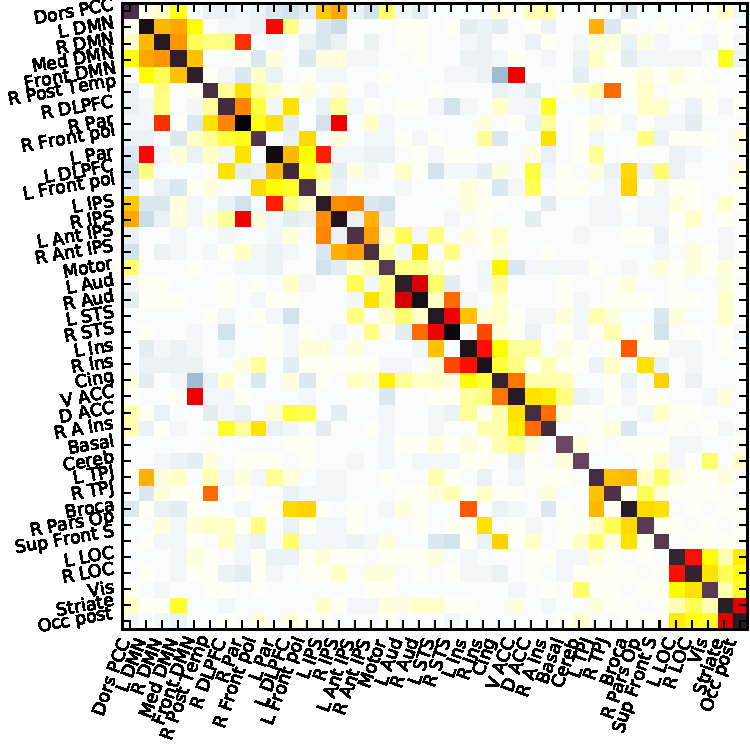
\includegraphics[width=\linewidth]{group_l21_prec.pdf}%
    \raisebox{.606\linewidth}{%
	\hspace*{-.462\linewidth}%
	\photoframe{%
	%\setlength\fboxsep{1pt}%
	\colorbox{white}{%
	\raisebox{.003\linewidth}{%
	    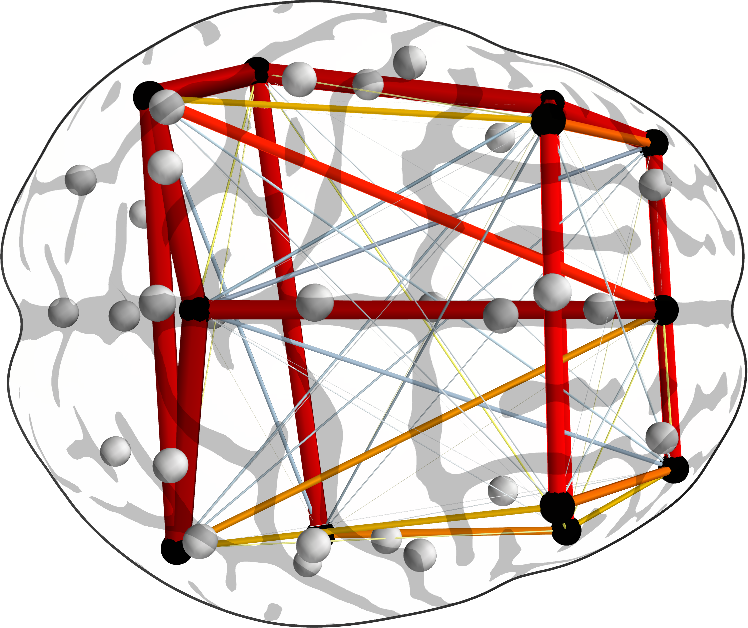
\includegraphics[width=.455\linewidth]{group_l21_prec_3d_crop}}%
	\rule{0pt}{.387\linewidth}%
	}}%
    }
\end{minipage}%
\hspace*{1pt}%
\begin{minipage}{.32\linewidth}%
    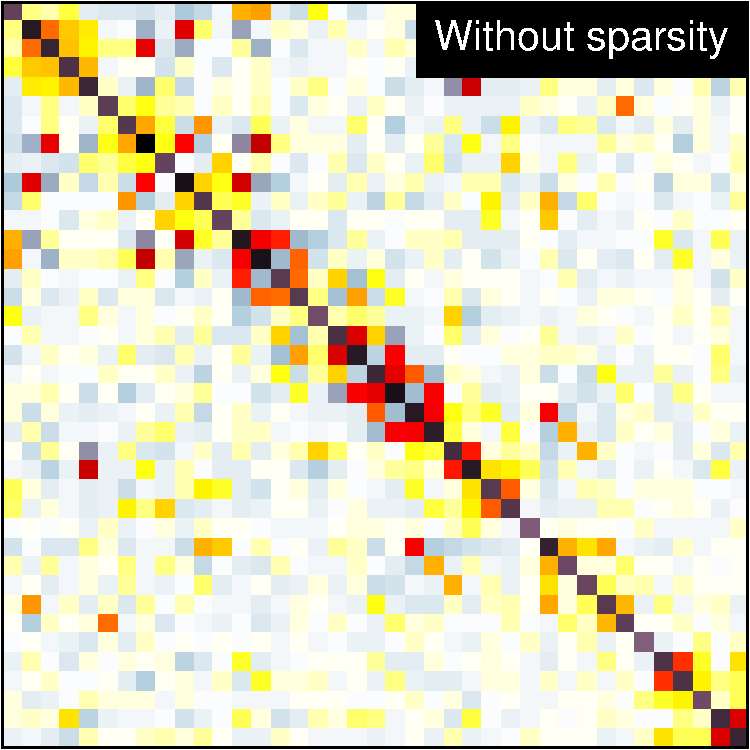
\includegraphics[width=\linewidth]{group_emp_prec.pdf}%

    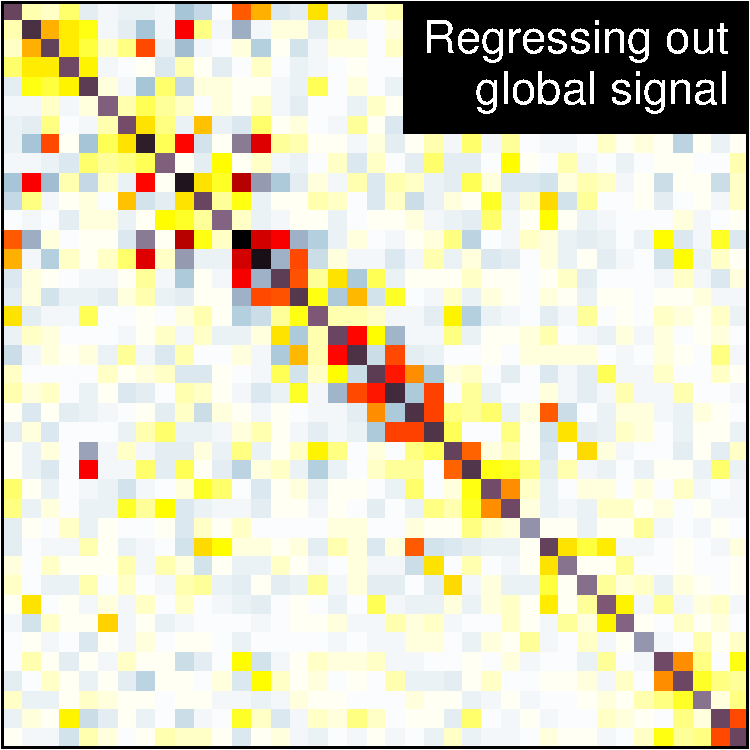
\includegraphics[width=\linewidth]{group_emp_prec_global_mean.pdf}%
\end{minipage}%

\caption{
Inverse-covariance matrices
}
\end{figure}
%---------------------------------------------------------------------------}}}

% XXX: should we have a summary paragraph commenting on the structure of
% the graphs and correlation matrices extracted.
% And also commenting on the meaning of regressions and sign of
% correlation coefficients (the whole global mean debate).
\cite{chai2011} (note: chai2011 used compcor)

%%%%%%%%%%%%%%%%%%%%%%%%%%%%%%%%%%%%%%%%%%%%%%%%%%%%%%%%%%%%%%%%%%%%%%%%%%%%%%%

\section{Comparing connections}

%------------------------------------------------------------------------------
\subsection{Mass-univariate approaches}

Boils down to a standard linear model => t-tests and co.
Stress that to have Gaussian-distributed correlations, a Fisher Z
transform is required.

Multiple comparison problem is quite an issue (scales a $p^2$) =>
permutation and max-T approach XXX: cite Ge
"resampling-based multiple testing for microarray data analysis", and
Nichols multiple comparison paper.

Family (Cameron, is that the correct name?) FWE?

%------------------------------------------------------------------------------
\subsection{Modeling between-connection dependences}

Show that correlations co-fluctuation with images, spatial correlations between correlations.

Ad-hoc model: network-based statistics \cite{zalesky2010}

Discuss the 'residual' strategy?
\cite{varoquaux2010b}

%%%%%%%%%%%%%%%%%%%%%%%%%%%%%%%%%%%%%%%%%%%%%%%%%%%%%%%%%%%%%%%%%%%%%%%%%%%%%%%

\section{Comparing Network Summary Statistics}

Small world networks, transport properties, resilient...

Warning note that correlation matrices have long-tailed degree
distribution by definition (cite recent Bullmore paper showing that).

Mutual information? Entropy correlation? MI as measure of integration (Marralec)

%%%%%%%%%%%%%%%%%%%%%%%%%%%%%%%%%%%%%%%%%%%%%%%%%%%%%%%%%%%%%%%%%%%%%%%%%%%%%%%

\section{Predictive Modeling}
craddock 2009, Dosenbach 2010, lord 2011, deshpande, 

1. importance of interpretation!
2. the need for feature extraction
3. the need for feature selection
4. setting parameters.
5. different methods have different interpretations

\emph{ --- CC text from TICS paper, do not use without modification!}
Multivariate Prediction Analysis. When applied to the study of intrinsic activity, the goal of discovery
science is to identify models that relate measures of that activity (such as iFC) to phenotypic variables.
Prediction analysis provides a means for measuring how well these models generalize to independent data.
This is complementary to inferential statistics, which measure the likelihood of such relationships
arising by chance. In the prediction analysis framework, a model relating iFC to a phenotype is learned 
from a training dataset. This model is then applied to an independent test dataset to predict phenotypes.
The resultant predictions are compared to the true phenotypes to estimate how well the model generalizes
to the tese dataset. Thus, prediction analysis provides a natural framework for evaluating biomarkers [21],
performing real-time fMRI [88], and evaluating experimental tradeoffs [89]. 

Prediction analysis has been applied to functional neuroimaging data since the early 90’s [90], and more
recently to IFC data [91]. Most, if not all, analysis methods can be applied in a predictive modeling
framework but the majority of methods that have been applied to iFC are multivariate classification and
regression methods (referred to as MVPA; multivariate prediction analysis). Multivariate methods are more
sensitive to distributed patterns of iFC than their univariate counterparts. Additionally they provide a
means for evaluating the significance of an entire pattern using a single statistic, obviating the need
to correct for multiple comparisons. 

Although there are many circumstances in which high prediction accuracy is the ultimate goal of an
analysis (e.g. predicting treatment outcome), in general it is desirable that the model also be
interpretable. Identifying the iFC measures (features) that are most important to the model is
problematic and an open issue for MVPA research. Several feature selection algorithms have been proposed
to address this issue, but there is no consensus on which is best [21]. We note that feature selection
methods that rely on feature-by-feature statistical tests require correction for multiple comparisons. 

MVPA classification has already been successfully used to identify potential iFC biomarkers of Alzheimer’s
disease [92], major depression [93], schizophrenia [94], and autism [47], among others. MVPA
classification and regression techniques have also been applied to identify biomarkers of age [95,96]
and recent work has shown the utility of MVPA methods for deriving iFC models at the individual
level [97]. An in-depth overview of the statistical pattern recognition methods underlying MVPA
techniques can be found in [98].
\emph{ --- END CC text from TICS paper, do not use without modification!}


%%%%%%%%%%%%%%%%%%%%%%%%%%%%%%%%%%%%%%%%%%%%%%%%%%%%%%%%%%%%%%%%%%%%%%%%%%%%%%%

\section{Functional and effective connectivity}

Effective connectivity does not have to be causal => but a precise mathematical
definition of the relationship => BCI workshop reports

Fucntional connectivity is a statistical relationship, instead of precise mathematical
relationship

%------------------------------------------------------------------------------
\subsection{From correlations to structural equation modeling}

\cite{mcintosh1994}
\cite{marrelec2007}
\cite{marrelec2009}

%------------------------------------------------------------------------------
\subsection{Matching model complexity to data}

Diatribe: all model are wrong, but some are useful => a cat is a model of a cat

Setting the cursor between complex models based on a bio-physical
description, and simple phenomenological models such as correlation
matrices.

\cite{mcintosh2010}

Cross validation???


%%%%%%%%%%%%%%%%%%%%%%%%%%%%%%%%%%%%%%%%%%%%%%%%%%%%%%%%%%%%%%%%%%%%%%%%%%%%%%%

\section{Conclusion}

{
%\clearpage
\section*{References} \small \bibliographystyle{elsarticle-num-names}
\bibliography{biblio} }

%%%%%%%%%%%%%%%%%%%%%%%%%%%%%%%%%%%%%%%%%%%%%%%%%%%%%%%%%%%%%%%%%%%%%%%%%%%%%%%


\end{document}
